%%%%%%%%%%%%%%%%%%%%%%%%%%%%%%%%%%%%%%%%%
% Short Sectioned Assignment
% LaTeX Template
% Version 1.0 (5/5/12)
%
% This template has been downloaded from:
% http://www.LaTeXTemplates.com
%
% Original author:
% Frits Wenneker (http://www.howtotex.com)
%
% License:
% CC BY-NC-SA 3.0 (http://creativecommons.org/licenses/by-nc-sa/3.0/)
%
%%%%%%%%%%%%%%%%%%%%%%%%%%%%%%%%%%%%%%%%%

%----------------------------------------------------------------------------------------
%	PACKAGES AND OTHER DOCUMENT CONFIGURATIONS
%----------------------------------------------------------------------------------------

\documentclass[paper=a4, fontsize=11pt, UTF8]{article} % A4 paper and 11pt font size
\usepackage[a4paper,left=3.18cm,right=3.18cm,top=2.5cm,bottom=2.5cm]{geometry}
\usepackage{ctex}
%\usepackage[T1]{fontenc} % Use 8-bit encoding that has 256 glyphs
%\usepackage{fourier} % Use the Adobe Utopia font for the document - comment this line to return to the LaTeX default
\usepackage[english]{babel} % English language/hyphenation
\usepackage{amsmath,amsfonts,amsthm} % Math packages
\usepackage{graphicx}
%\usepackage{rotating} % for sidewaysfigure
\usepackage{listings}
\usepackage{xcolor}
\usepackage{siunitx}
\usepackage{booktabs}
\usepackage{multirow}
\usepackage{longtable}
\usepackage{hyperref}
\hypersetup{
    colorlinks,
    citecolor=black,
    filecolor=black,
    linkcolor=black,
    urlcolor=black
}

% Uncomment below to New page befor section
%\usepackage{titlesec}
%\newcommand{\sectionbreak}{\clearpage}
%\titleformat*{\section}{\centering \Large \bfseries}

\newcommand{\matr}[1]{\mathbf{#1}} % undergraduate algebra version
%\usepackage{sectsty} % Allows customizing section commands
%\allsectionsfont{\centering \normalfont\scshape} % Make all sections centered, the default font and small caps

\usepackage{fancyhdr} % Custom headers and footers
\pagestyle{fancyplain} % Makes all pages in the document conform to the custom headers and footers
\fancyhead[L]{}
\fancyhead[C]{}
\fancyhead[R]{\thepage} % No page header - if you want one, create it in the same way as the footers below
\fancyfoot[L]{} % Empty left footer
\fancyfoot[C]{\thepage} % Empty center footer
\fancyfoot[R]{} % Page numbering for right footer
%\renewcommand{\headrulewidth}{0pt} % Remove header underlines
\renewcommand{\footrulewidth}{0pt} % Remove footer underlines
\setlength{\headheight}{13.6pt} % Customize the height of the header

\numberwithin{equation}{section} % Number equations within sections (i.e. 1.1, 1.2, 2.1, 2.2 instead of 1, 2, 3, 4)
\numberwithin{figure}{section} % Number figures within sections (i.e. 1.1, 1.2, 2.1, 2.2 instead of 1, 2, 3, 4)
\numberwithin{table}{section} % Number tables within sections (i.e. 1.1, 1.2, 2.1, 2.2 instead of 1, 2, 3, 4)

%\setlength\parindent{0pt} % Removes all indentation from paragraphs - comment this line for an assignment with lots of text

\lstset{language=Python,%
    %basicstyle=\color{red},
    keywordstyle=\color{blue},%
    extendedchars=false,
    breaklines,
    identifierstyle=\color{black},%
    stringstyle=\color{red},
    commentstyle=\color{green},%
    frame=single,
    showstringspaces=false,%without this there will be a symbol in the places where there is a space
    numbers=left,%
    numberstyle={\small \color{black}},% size of the numbers
    numbersep=9pt, % this defines how far the numbers are from the text
    emph=[1]{for,end,break},emphstyle=[1]\color{red}, %some words to emphasise
    escapeinside=``
}


\newcommand{\horrule}[1]{\rule{\linewidth}{#1}} % Create horizontal rule command with 1 argument of height

\title{
\normalfont \normalsize
\textsc{\kaishu 搜索引擎技术基础} \\ [5pt] % Your university, school and/or department name(s)
\horrule{0.5pt} \\[0.4cm] % Thin top horizontal rule
\huge 校园搜索引擎构建 \\ % The assignment title
\horrule{2pt} \\[0.5cm] % Thick bottom horizontal rule
}

\author{马\; \, 也 \quad 2013011365 计34 \\ 刘政宁 \quad 2013011362 计34}
%\author{马也} % Your name
\date{\normalsize\today} % Today's date or a custom date

\begin{document}

\maketitle % Print the title

\thispagestyle{empty}
\newpage

\setcounter{page}{1}
%\tableofcontents
\fontsize{10pt}{15pt}\selectfont
%\newpage

\section{实验要求和内容}

本项目要求综合运用搜索引擎体系结构和核心算法方面的知识,基于开源资源搭建校园搜索引擎,掌握开源搜索引擎的运行流程。具体要求为:

\begin{enumerate}
\item 抓取清华校内绝大部分(30万左右)网页资源及大部分在线文本资源(如office文档、pdf文档等)
\item 实现基于BM25概率模型的内容排序算法,要求对查询进行分词;
\item 实现基于HTML结构的分域权重计算(content/title/h1-h6),并应用到搜索结果排序之中,并建立小规模测试集合,进行参数调节;
\item 实现基于Page Rank的连接结构分析功能,离线计算Page Rank值,并应用到搜索结果排序之中;
\item 采用便于用户信息交互的Web界面,实现查询扩展、查询纠错等功能。
\end{enumerate}


\section{实验功能}

本项目在全部完成基础要求的同时,最终完成如下扩展功能,具体功能描述及效果参见实验成果一节。

\begin{itemize}
\item 基于HTML结构的分域权重计算(包含content/title/h1-h6等),不同域权值不同
\item 实现了条件查询功能,即支持不同查询语句的AND、OR、NOT组合
\item 实现了模糊查询功能,即支持自动纠正错误输入,并得到正确查询结果
\item 实现了通配符查询(正则表达式)功能,即支持* ? \^  等通配符进行查询
\item 实现了查询特定范围功能,即支持查询某一网域下的相关网页
\item 实现了查询特定类型功能,即支持查询某一或某几类型的资源
\item 实现了查询结果界面的高亮处理,即找到最佳高亮位置,显示到摘要之中
\item 实现了对特定HTML结构的查询,即支持仅在标题、h1等结构中查询
\end{itemize}

\section{实验框架及运行环境}

\subsection{框架概要}

\begin{figure}[htp]
\center
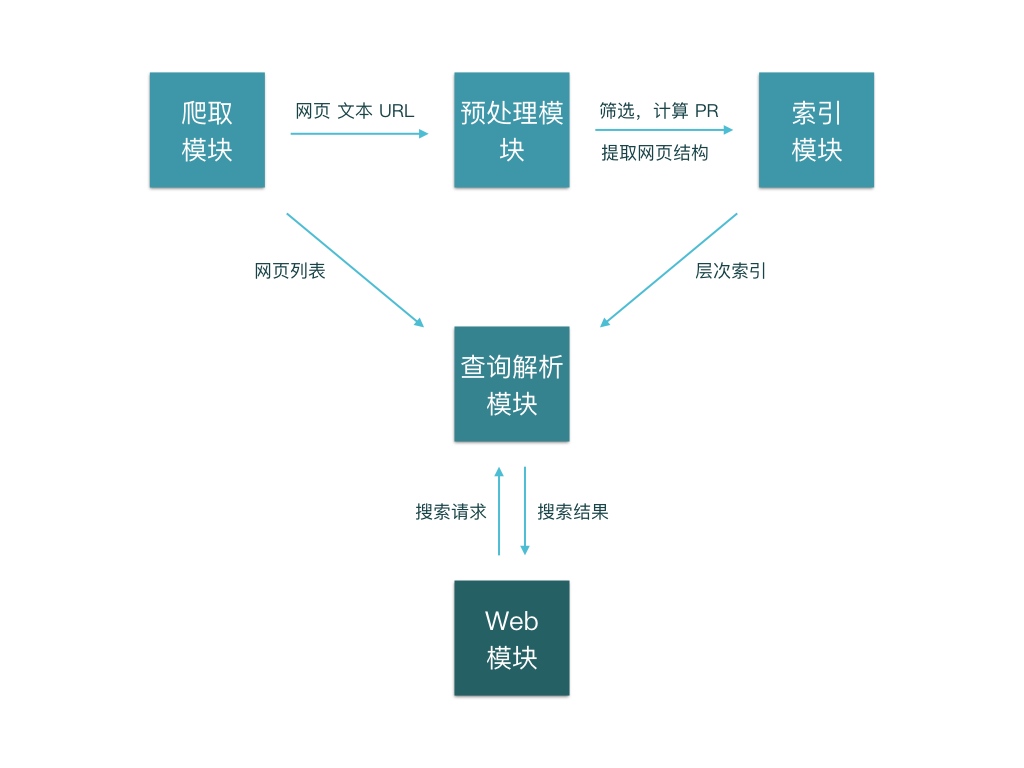
\includegraphics[width=\textwidth]{arch}
\caption{实验框架} \label{relation}
\end{figure}

本项目主要分为五个模块:爬取模块、预处理模块、索引模块、查询解析模块以及Web模块。主要流程关系参见图\ref{relation},具体阐述如下:

\textbf{爬取模块}从清华校内爬取网页和文本数据,并按照网页结构(url)分文件夹存放在本地,对应搜索引擎中的数据抓取子系统;

\textbf{预处理模块}分析和处理爬虫爬取到的数据,筛选高质量网页,提取网页HTML结构到纯文本文件之中,交由索引模块使用,并分析网页链接结构,计算Page Rank值,其对应搜索引擎中的链接分析子系统和内容索引子系统的一部分;

\textbf{索引模块}则利用预处理模块提取好的文本文件,使用分词器构建多层次索引,存储各层结构的文本信息到索引数据库中,以备查询模块使用,其对应搜索引擎中的内容索引子系统;

\textbf{查询解析}模块利用建立好的索引,根据查询条件和要求构建相应的查询语句,分拆高级查询语句为基本查询语句的组合,并在索引数据库中进行查询,返回查询到的文档列表,其对应内容检索子系统;

\textbf{Web模块}代表了搜索引擎所对应的网站,其负责接收用户请求,发送给查询解析模块,收到结果后以合理的格式与结构返回给用户。

\subsection{爬取模块}

爬取模块使用第三方库Heritrix 3.2.0完成,Heritrix可以对抓取的对象进行精确的控制,很好地符合我们校园搜索的要求。需要指出的是,最早项目使用课件上使用的版本,但其爬取速度太慢,且正则表达式过滤模块有隐含的BUG,所以最终替换为更新的版本,因此配置和课件上的配置有所不同。主要配置了如下内容:

\begin{itemize}
\item 种子资源:http://news.tsinghua.edu.cn/
\item 接受网页总规则:以tsinghua.edu.cn结尾,且不以lib.tsinghua.edu.cn结尾,不属于166.111.120网段
\item 拒绝类型规则:js|JS|axd|AXD|mso|tar|txt|asx|asf|bz2|mpe?g|MPE?G|tiff?|gif等,从略
\end{itemize}

除此之外,还设置了爬取速度,最大条数等具体配置,最终爬取了40万以上的文件,删除掉其中大于32M的较大文件,最终剩余35万左右。

\subsection{预处理模块}

预处理模块基本使用Python 3 完成,计算Page Rank使用C++完成,代码在preprocess文件夹内,脚本文件及对应功能如下:

\begin{itemize}
\item \textbf{parse\_log.py}:分析Heritrix日志,建立文件名到网页URL的双向映射关系
\item \textbf{get\_id.py}:分析链接结构,筛选有效网页,给每个网页分配独立id,并得到链接图谱
\item \textbf{append\_id.py}:对get\_id的补充
\item \textbf{prepare\_pr.py}:将Python结构按照规则写入文件,为C++程序准备输入
\item \textbf{page\_rank.cc}:计算Page Rank,写入文件中,每行一个id和对应的Page Rank
\item \textbf{get\_text.py}:提取网页文本内容,删除script、css以及HTML标记,每个网页存入一个文本文件中,文件名为网页id
\item \textbf{get\_title.py}:提取网页标题(<title>域),写入文件中,每行一个id和对应的title
\item \textbf{get\_file\_text.py}:提取PDF、DOC、DOCX等格式的全部文本,每个文件存入一个文本文件中
\item \textbf{get\_file\_title.py}:提取PDF文件的标题,写入文件中,每行一个id和对应的title
\item \textbf{ get\_docs\_title.py}:提取WORD文件的标题,写入文件中,每行一个id和对应的title
\item \textbf{get\_h1.py}:提取网页结构,(h1-h6),分别写入文件中
\end{itemize}

需要注意的是,由于Heritrix在抓取带GET请求的网页时,存储文件的文件名和网址URL并不能一一对应(其去掉了问号,挪动了文件类型的位置),且单从文件名并不能找到对应的URL,所以第一步分析Heritrix爬取日志是必要且是必须的。通过分析日志,得到了URL到文件名的双向映射,同时删除了404网页,将网页个数减少到32万左右。

以上处理中对于HTML网页的处理使用Beautiful Soup完成,其负责提取链接关系,提取文本信息,提取title和提取h1-h6域等,部分编码混乱的网页被直接丢弃,将网页个数再减到30万左右。

另外,由于绝大多数下载附件网页的文件名都是数字编号或无意义符号,所以提取PDF和DOC文件的标题也是十分重要的。提取PDF内容使用了pdftotext程序,提取PDF标题使用了pyPdf库,通过PDF文件的Meta信息能够得到大部分PDF的准确文件名,提取DOC文件使用了antiword程序,提取DOCX文件使用了docx库。

\subsection{索引模块}

索引模块使用Lucene 5.5完成(MyIndexer.java),主要存储了网页id、网页标题、网页内容(content/h1-h6等)、网页类型(HTML/WORD/PDF等)、网页Page Rank值到索引之中,其中网页标题、内容进行了分词处理,分词时使用了效果更好的jcseg第三方库,可以有效地区分数字、人名、专有名词等,分词准确率更高。

索引时使用的评分模块为BM25模型的改版(MySimilarity.java),BM25模型在Lucene 5.5官方提供的BM25Similarity的基础上进行了重构,加入了Page Rank的计算,修改了最终得分公式,将BM25的得分与Page Rank的0.5次方乘起来得到最终得分,最终评分公式为:

$$
\mathrm{Score} =  \mathrm{idf} \cdot \dfrac{(k + 1) \cdot \mathrm{freq}}{k \cdot (1 - b + b \cdot \frac{|d|}{\mathrm{avgLen}}) + \mathrm{freq}} \cdot \sqrt{\mathrm{PageRank}}
$$

这里使用根号的原因是减少Page Rank对于结果的影响,因为Page Rank范围变化较大($10^{-{3}}$ 到 $10^{-{7}}$),如果直接将BM25结果和Page Rank结果相乘,会导致Page Rank高的网页,即使只出现一次也会排名非常靠前,这就让BM25算法失去了意义。

\subsection{查询解析模块}

查询解析模块使用Lucene 5.5完成(MySearcher.java),主要实现了普通搜索(search())、获得文本高亮(getHighlight())、高级搜索(searchComplex())、通配符和模糊搜索(searchFuzzy OrWildCard())等功能。

需要注意的是,如果直接使用QueryParser,其生成的Query语句的分词间是SHOULD的关系,即只要有一个出现即可,这不太符合大多数搜索的要求,如搜索“清华大学计算机系”时可能出现只含“清华大学”而不含“计算机系”的文档,所以要使用QueryBuilder类的createMinShouldMatch方法构建Query,这样保证分词后的每个词都必须出现,而不是出现一个即可。

得到了基础的Query之后,需要根据要求再不同域上进行搜索(content、title、h1、type等),并且需要使用BoosQuery提供不同域的不同权值。如果进行条件搜索,则需要BooleanQuery对其进行组合,BooleanQuery中的SHOULD、MUST、MUST\_NOT分别对应OR、AND和NOT。

对于通配符搜索和模糊搜索,则可以使用WildCardQuery和FuzzyQuery,按照类似的要求进行组合,得到最终的Query查询。

文本高亮也是在这一模块实现的,主要使用Lucene中的Highlighter类,对于一个特定的Query、特定的field和和内容,可以找到最佳的文本段,其出现特定关键词的次数最多、得分最高,将其返回给前端,就可以实现类似于Baidu、Google等搜索引擎的文本高亮了。

\subsection{Web模块}

该模块使用Tomcat服务器完成(IndexServlet.java和ResultServlet.java),主要实现了myIndex.jsp和myResult.jsp两个动态页面,其负责显示搜索结果,进行分页处理等操作,并接受用户高级搜索的输入,转化为查询解析模块的函数调用。


\section{实验成果与分析}

\subsection{主要功能与效果图}

\subsubsection{主界面}

\begin{figure}[htp]
\center
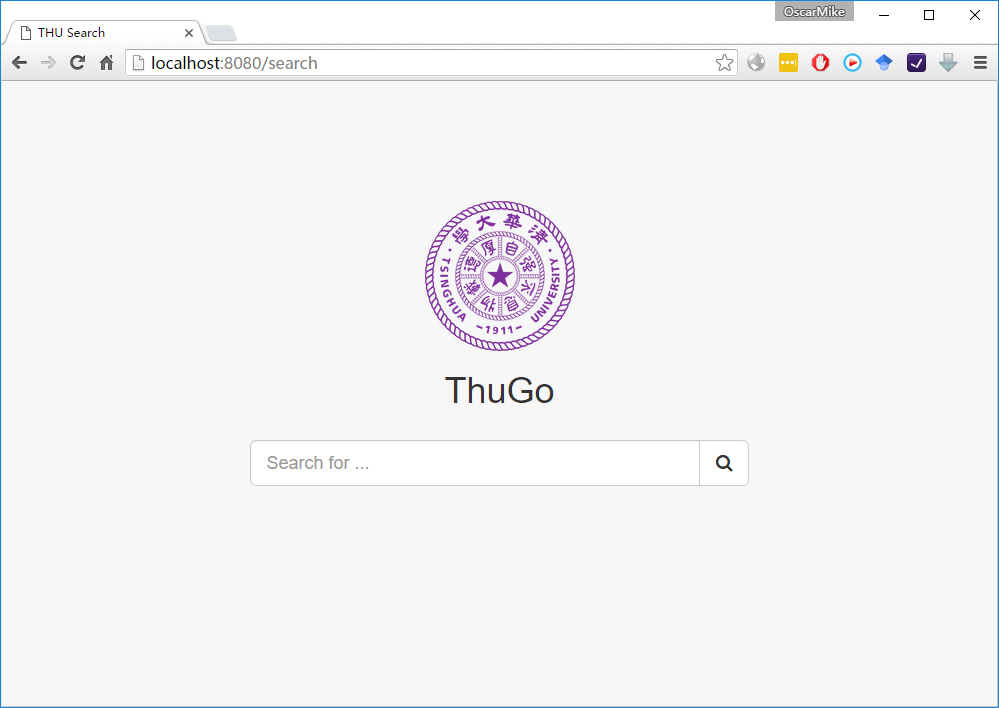
\includegraphics[width=\textwidth]{ss1}
\caption{主界面} \label{ss1}
\end{figure}

如图\ref{ss1}所示为简单大方的主界面。

\subsubsection{搜索结果页面}

\begin{figure}[htp]
\center
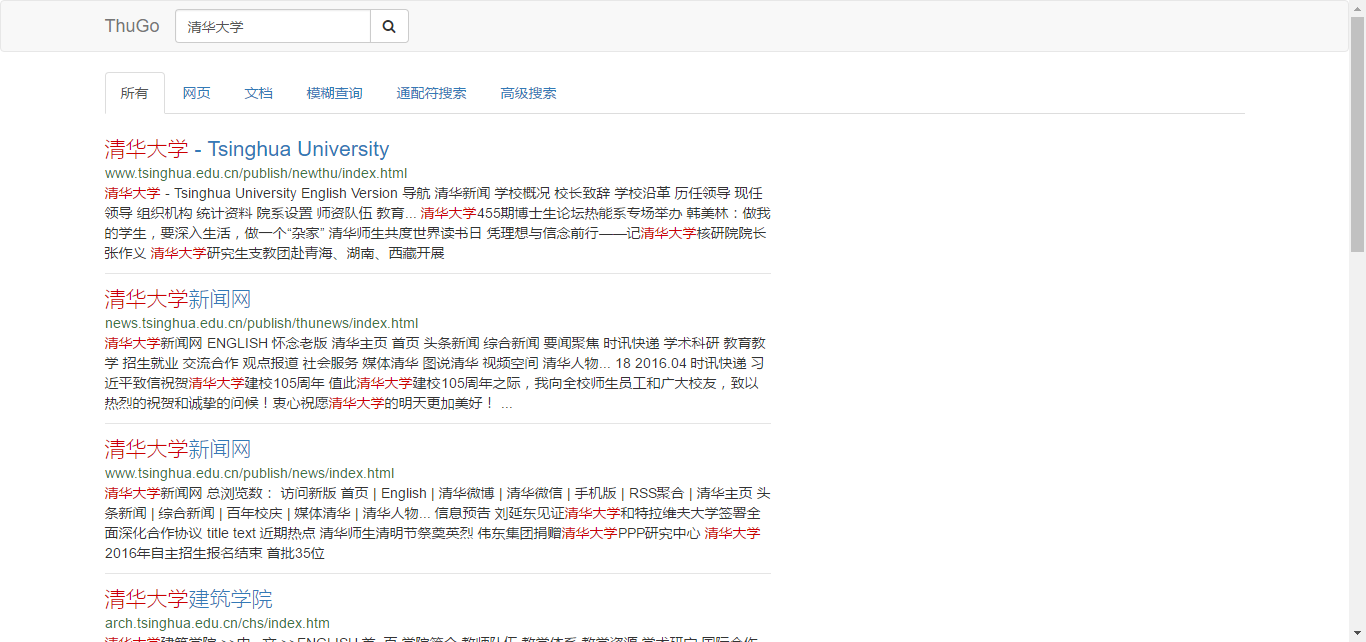
\includegraphics[width=\textwidth]{ss2}
\caption{搜索结果} \label{ss2}
\end{figure}

如图\ref{ss2}所示为搜索“清华大学”的结果,可以看出标题和摘要中都带有高亮处理,可以让人对网站内容有一个初步的了解。

\subsubsection{搜索文件功能}

\begin{figure}[htp]
\center
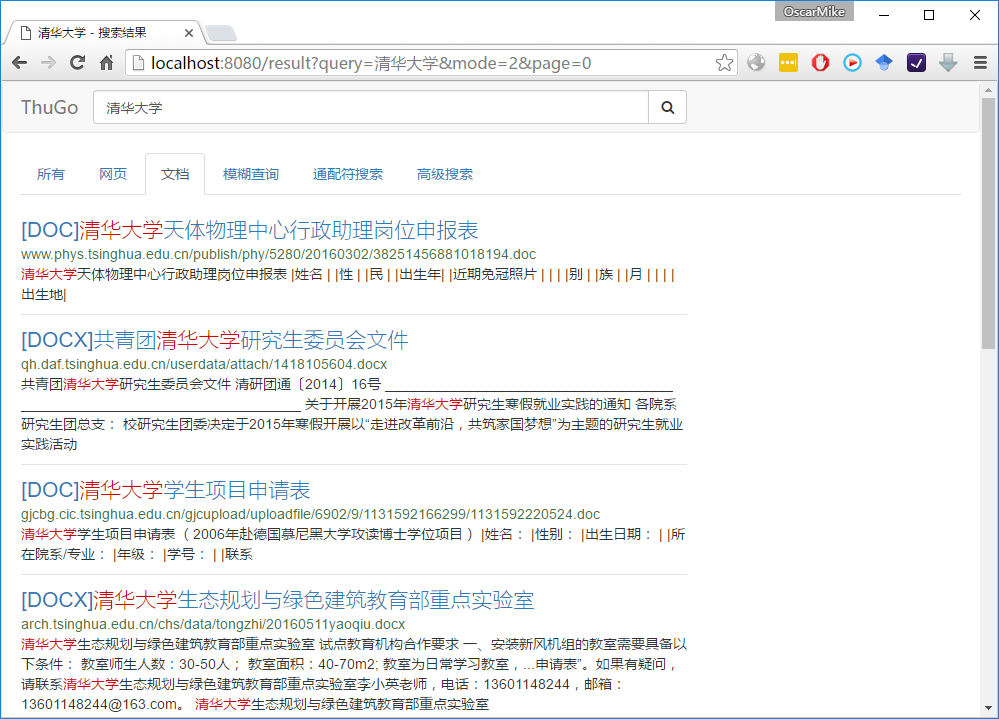
\includegraphics[width=\textwidth]{ss3}
\caption{仅搜索文件功能} \label{ss3}
\end{figure}

如图\ref{ss3}为搜索“清华大学”,并且只要非HTML格式的文件,返回的搜索结果,可以看到非HTML的标题提取也都基本正确,并且摘要信息基本符合要求。

\subsubsection{模糊搜索功能}

\begin{figure}[htp]
\center
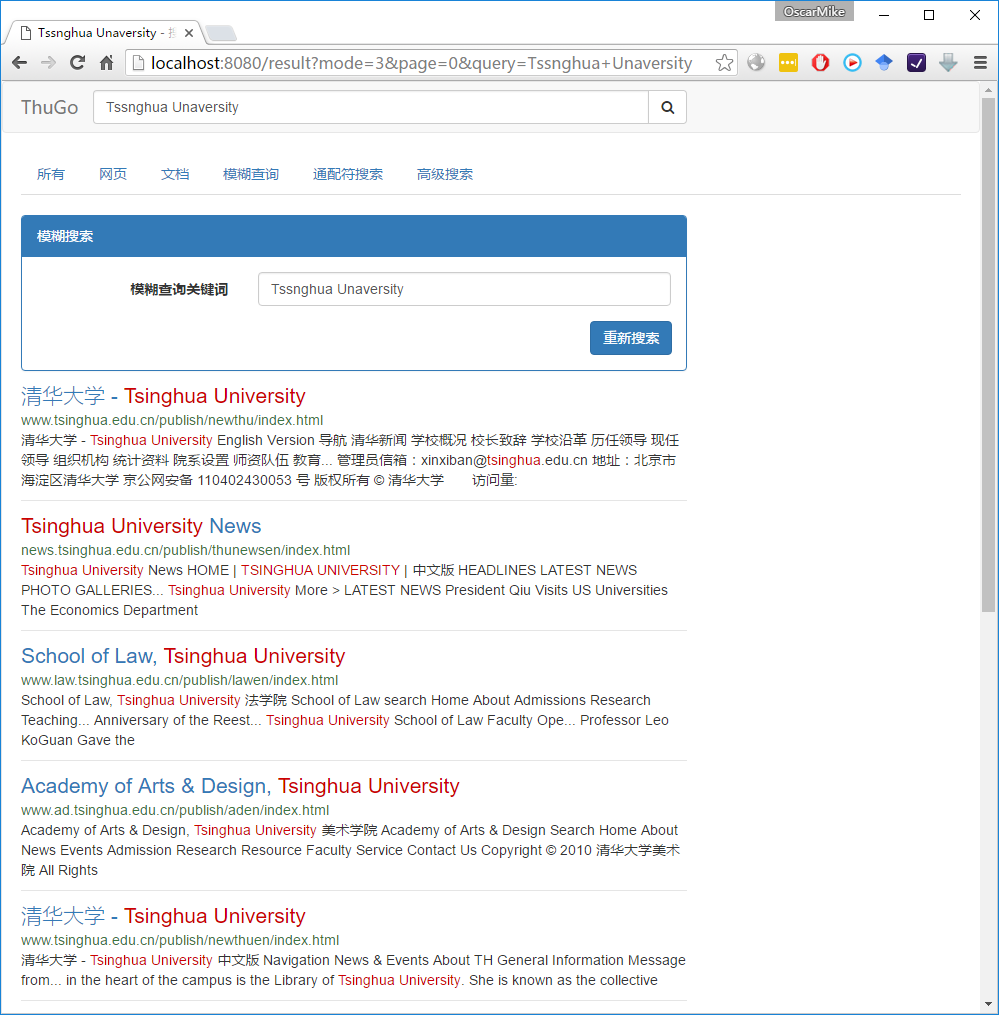
\includegraphics[width=\textwidth]{ss4}
\caption{模糊搜索功能} \label{ss4}
\end{figure}

如图\ref{ss4}为搜索Tssnghua Unaversity这一错误查询时返回的结果,可以看到其自动更正为Tsinghua University,并且正确的进行了高亮。

\subsubsection{通配符搜索功能}

\begin{figure}[htp]
\center
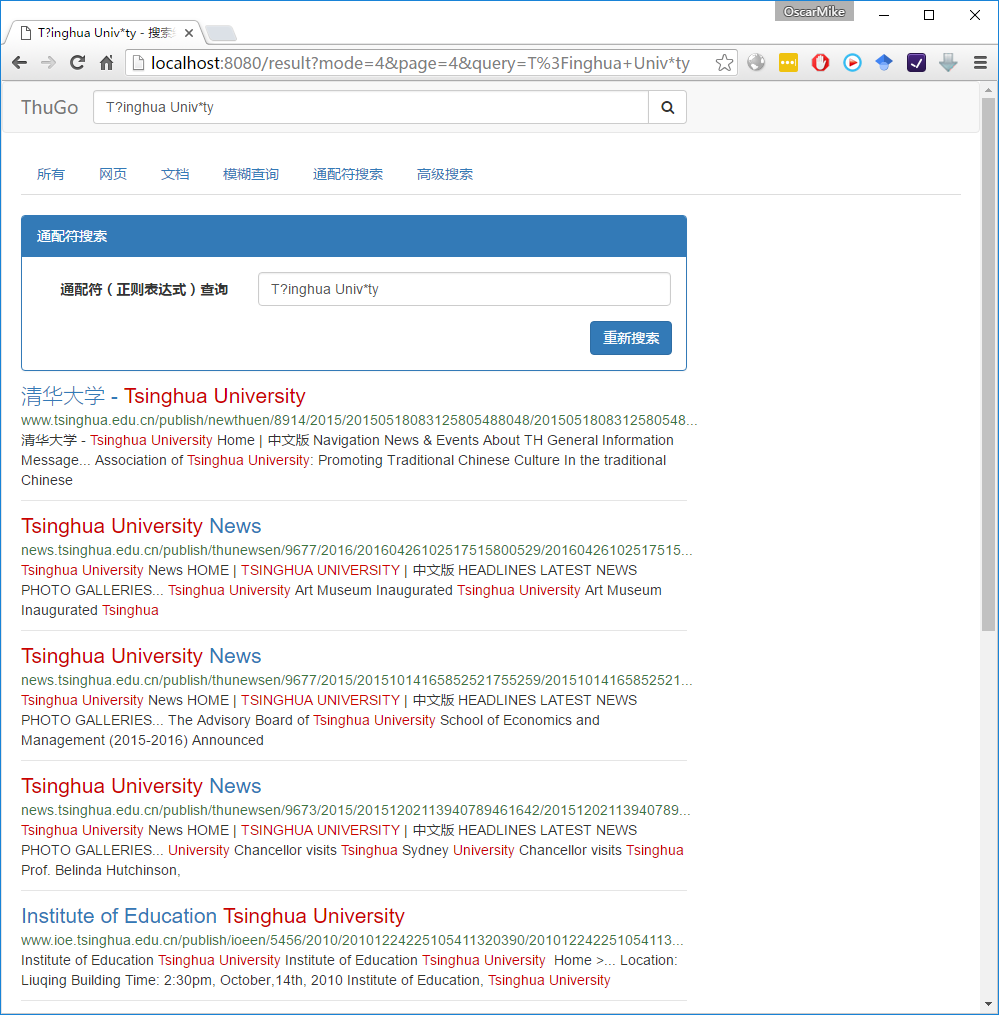
\includegraphics[width=\textwidth]{ss5}
\caption{通配符搜索功能} \label{ss5}
\end{figure}

如图\ref{ss5}为搜索T?inghua Univ*ty这一带通配符查询时返回的结果,可以看到其匹配到了Tsinghua University,并且正确的进行了高亮。

\subsubsection{条件搜索功能}

如图\ref{ss6}为高级搜索的界面,其支持如下功能:

1. 包含\textbf{全部}关键词的搜索(即每个词都要出现)

2. 包含\textbf{任意}一个或多个关键词的搜索(即所有词至少出现一次)

3. \textbf{不包含}任何一个关键词的搜索(即所有词都不能出现)

4. 限定搜索所在的\textbf{网域},如只搜索www.cs.tsinghua.edu.cn网域下的所有网页

5. 限定搜索文档的\textbf{格式}:PDF、DOC、DOCX、HTML等

6. 限定关键词在文档中出现的\textbf{位置}:全部、仅出现在标题、仅出现在h1等

7. 以上6点搜索的任意组合

\begin{figure}[htp]
\center
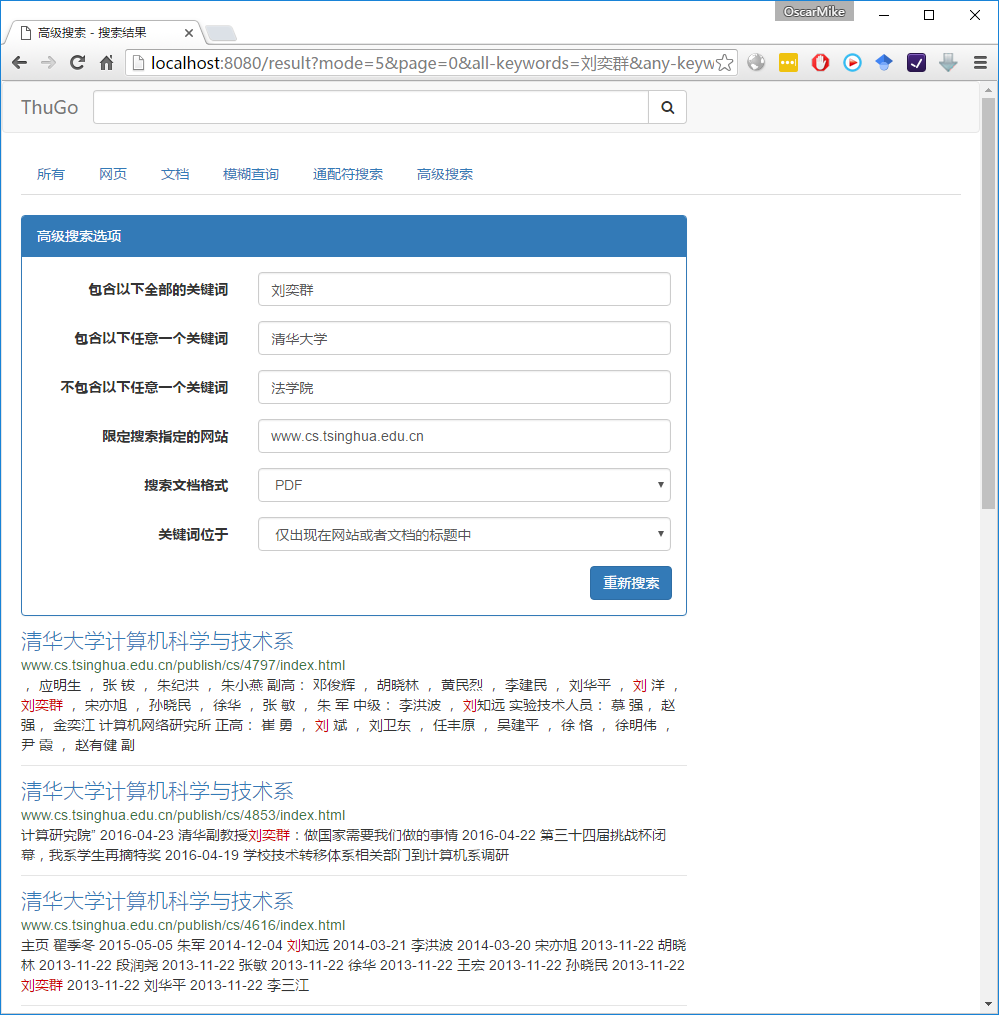
\includegraphics[width=\textwidth]{ss6}
\caption{高级搜索功能} \label{ss6}
\end{figure}

\subsection{实验结果分析}

\subsubsection{入链接、出链接分布}

首先,对抓取到的网页进行入链接、出链接统计,可以得到它们的分布情况,如下图所示:

\begin{figure}[htp]
\center
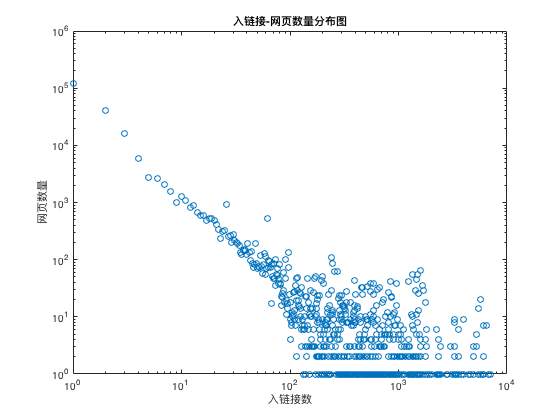
\includegraphics[scale=0.5]{in_degree}
\caption{入链接分布情况}
\end{figure}

\begin{figure}[htp]
\center
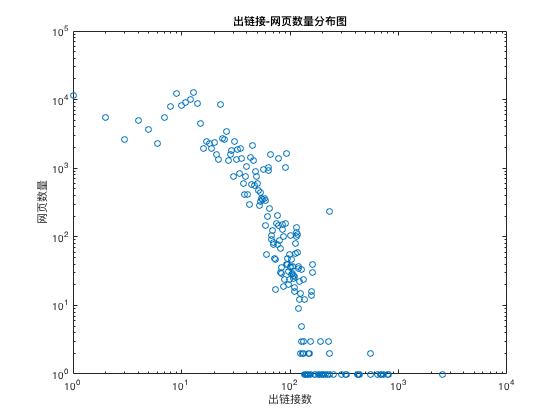
\includegraphics[scale=0.5]{out_degree}
\caption{出链接分布情况}
\end{figure}

从中我们可以看出,对于入链接个数分布情况来说,较好的满足了幂律,即入度与出现次数满足指数函数关系;而对于出链接个数分布来看,其在低频区不能很好的满足幂率,但是依然有着相似的分布。

\newpage
\subsubsection{PageRank算法结果}

接着,我们计算爬取所有网页的Page Rank,并把前20名列举如下:

\begin{table}[htp]
\centering
\begin{tabular}{@{}lcc@{}}
\toprule
内容                   & 入度   & Page Rank \\ \midrule
环境资源能源法学院 - 评论栏      & 2007 & 0.004005  \\
清华启航网 - 岗位列表         & 6518 & 0.003324  \\
清华启航网 - 基地列表         & 6518 & 0.003324  \\
清华启航网 - 首页           & 6518 & 0.003298  \\
环境资源能源法学院 - 评论栏      & 2008 & 0.003085  \\
清华启航网 - 联系方式         & 6518 & 0.002955  \\
清华启航网 - 企业服务         & 6518 & 0.002955  \\
清华启航网 - 平台介绍         & 6518 & 0.002955  \\
清华启航网 - 学生实践反馈       & 6518 & 0.002955  \\
环境资源能源法学院 - 评论栏      & 3    & 0.001818  \\
清华大学研究生院 - 首页        & 2744 & 0.001672  \\
清华大学深研院院报 - 首页       & 3144 & 0.001305  \\
清华大学建筑学院 - 首页        & 529  & 0.001280  \\
清华大学新闻网 - 首页         & 7034 & 0.001261  \\
清华大学美术学院 - 首页        & 4402 & 0.001208  \\
清华大学新闻网 - 英文版首页      & 6765 & 0.001179  \\
清华大学美术学院 - 英文版首页     & 4405 & 0.001131  \\
清华大学新闻网 - 旧版首页       & 6752 & 0.001085  \\
实验室管理系统 - 首页         & 3253 & 0.001077  \\
清华大学新闻网 - 首页(url重定向) & 1758 & 0.001058  \\ \bottomrule
\end{tabular}
\caption{前20名Page Rank结果}\label{table1}
\end{table}

从结果中,我们发现,尽管像清华新闻网首页和一些院系首页进入了前20名,但是排名靠前的却都是一些内容极其差的网页,例如环境资源能源法学院评论栏中都是些奇怪的文本,且评论栏有上千页写死到网站HTML之中,所以入度较高;又如清华启航网,他的网页个数极多,且都是测试使用的网站。由此可见,这些垃圾网页都是靠着极多的互相链接关系,形成一个很大的闭环,并不代表网站质量很高。基于以上考虑,最终部署时,已将这些垃圾网页去除。

\begin{figure}[htp]
\center
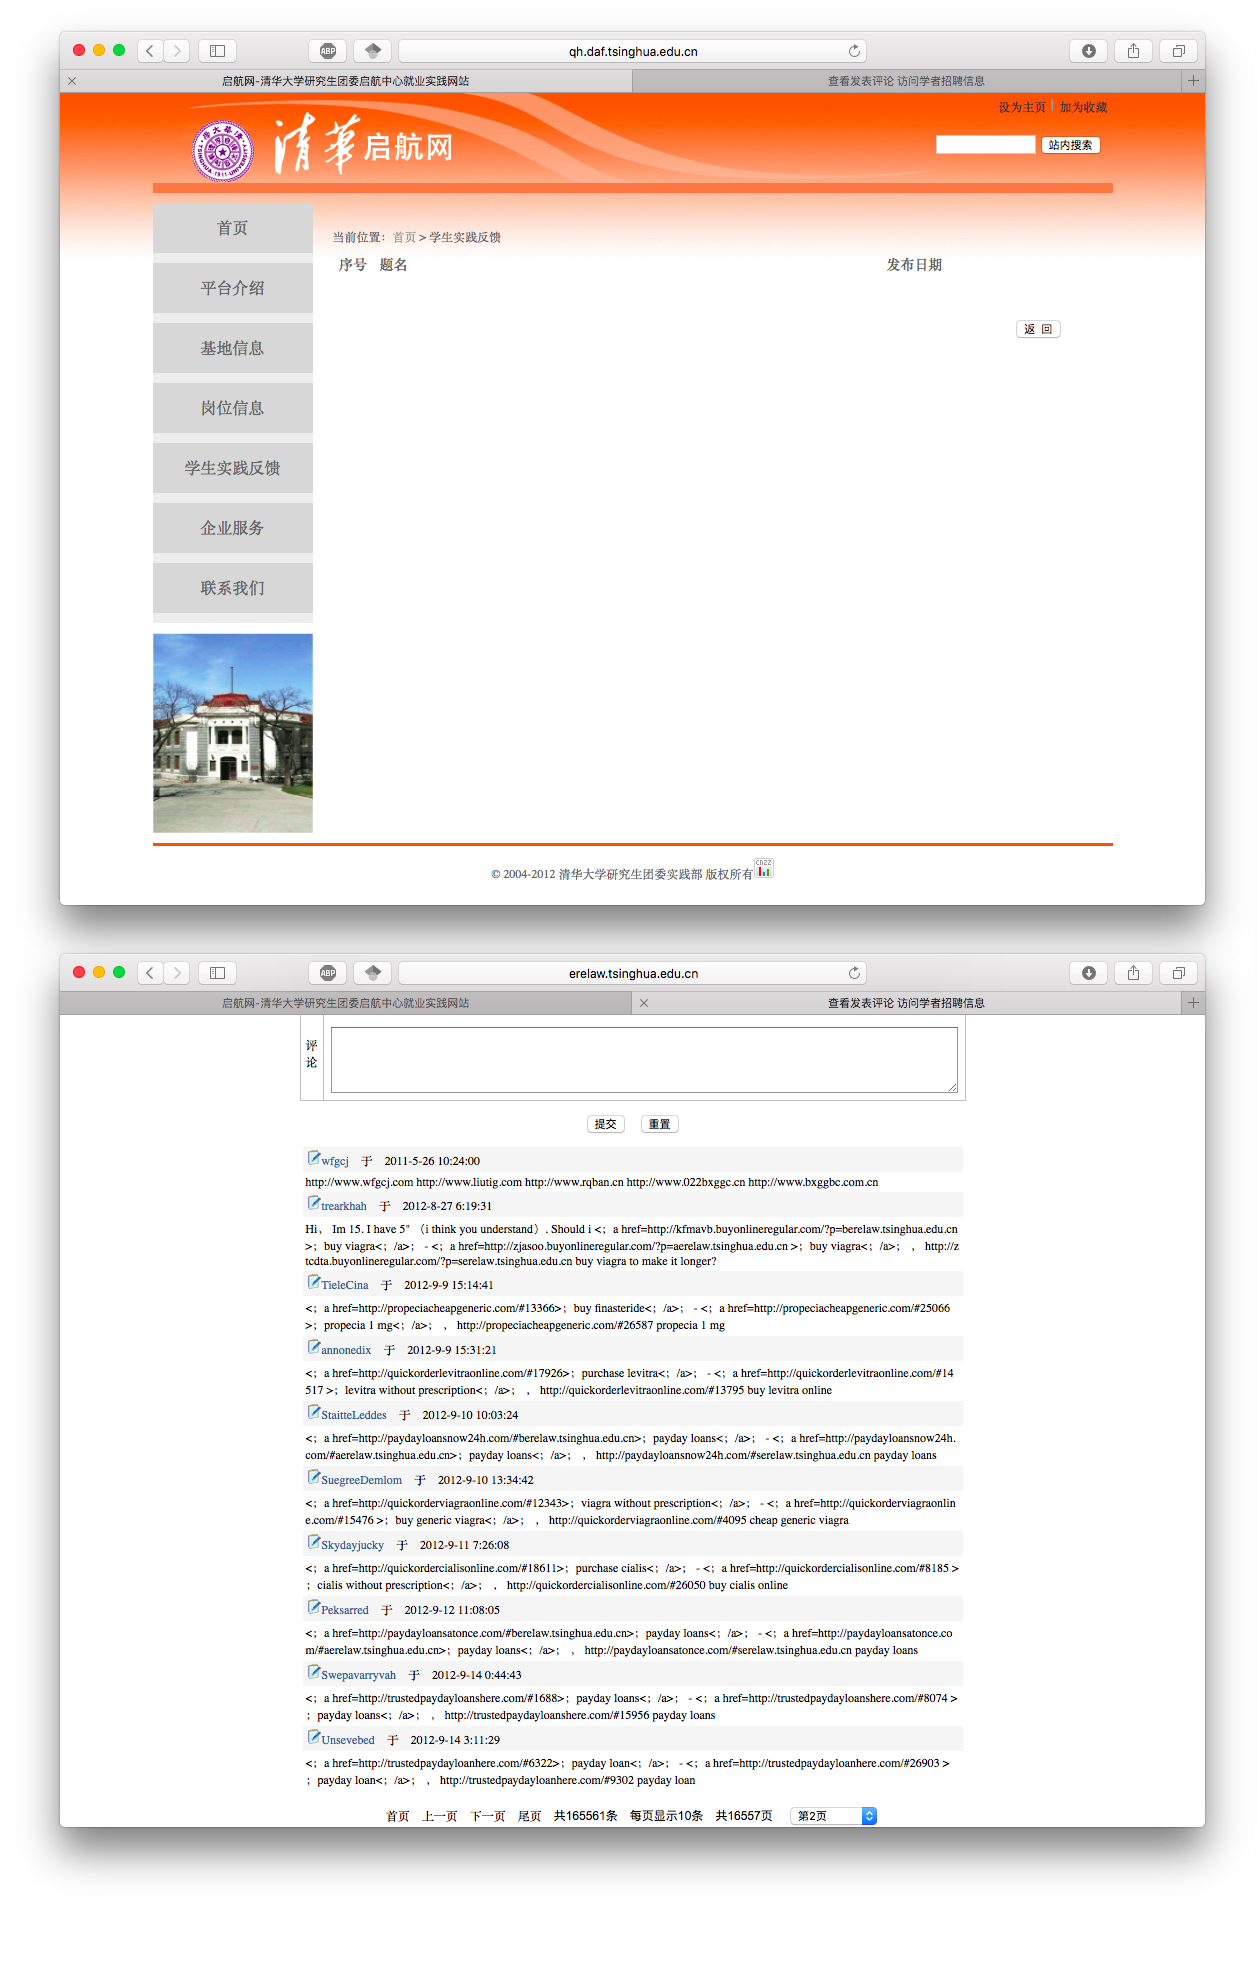
\includegraphics[width=\textwidth]{ss0}
\caption{部分垃圾网页截图} \label{ss0}
\end{figure}

\newpage

\subsubsection{PageRank结果分布情况}

接着,我门分析了Page Rank结果的分布情况,绘制如下图表:

\begin{figure}[htp]
\center
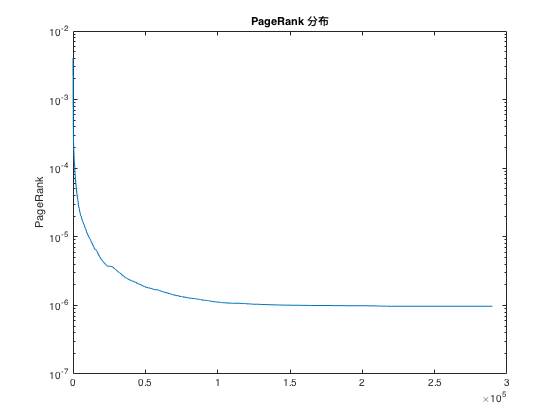
\includegraphics[scale=0.5]{pr}
\caption{PageRank结果分布情况}
\end{figure}

其中横轴为倒序排布后网站编号,纵轴为Page Rank值的以10为底的对数值。从图中我们可以发现,Page Rank值的衰减是非常非常快的。

\subsubsection{PageRank与入链接数的关联分析}

如果画出Page Rank和入链接数的散点图,我们可以得到如下结果:

\begin{figure}[htp]
\center
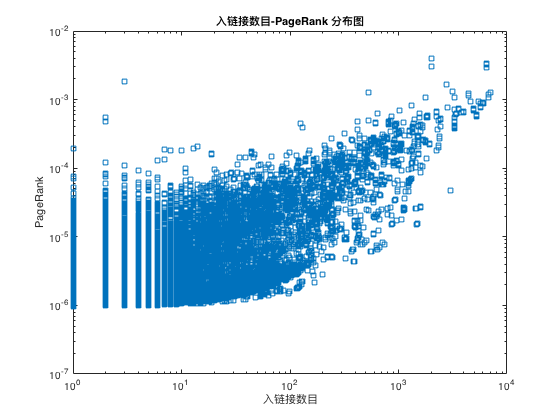
\includegraphics[scale=0.5]{pr_in_degree}
\caption{PageRank与入链接数的关联分析}
\end{figure}

其中横轴是入链接数以10为底的对数坐标,纵轴是Page Rank以10为底的对数坐标。从图中我们可以发现,尽管二者并不是严格的正相关,但是随着入度的增加,Page Rank是有增加的趋势的。

\subsubsection{搜索结果得分}

在调试过程中,我们经常需要知道一个页面排名靠前的原因,因此得分的计算过程就显得尤为重要了。在我们实现的MySimilarity中,就提供了explain的接口可以解释得分的来龙去脉,以搜索“相声”为例,排名前3的网页如下所示:

\begin{figure}[htp]
\center
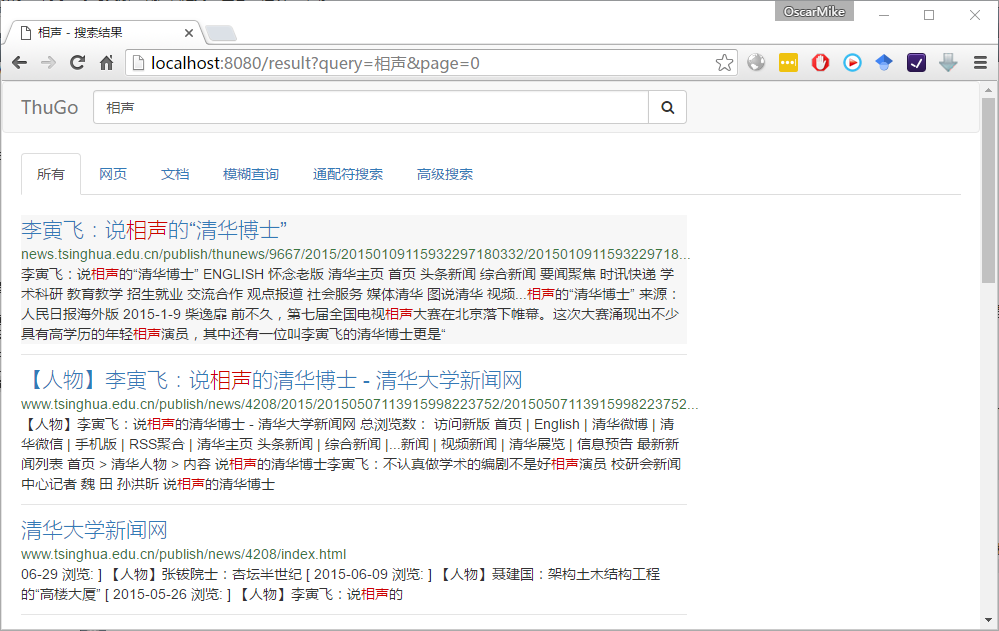
\includegraphics[width=\textwidth]{ss7}
\caption{“相声”搜索结果} \label{ss7}
\end{figure}

接下来我们分别导出前三名网页的得分及其来源

\begin{figure}[htp]
\center
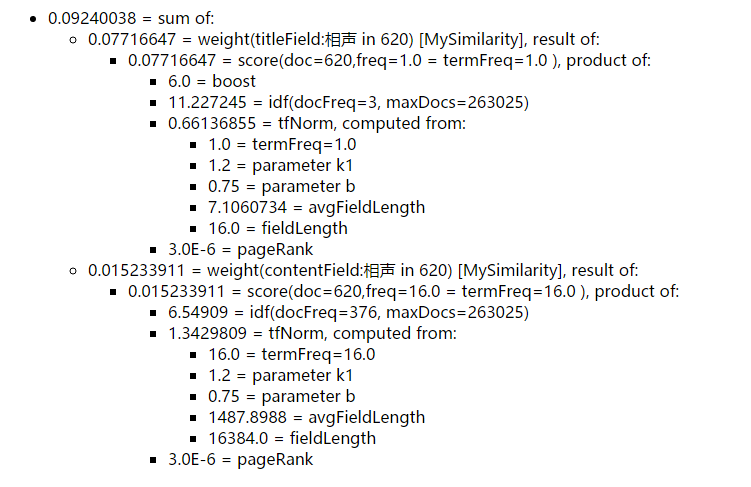
\includegraphics[scale=0.5]{t1}
\caption{排名第一的得分情况}
\end{figure}

\begin{figure}[htp]
\center
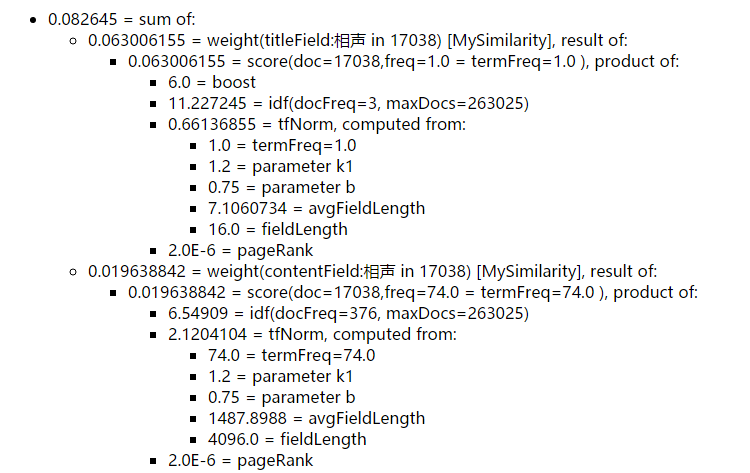
\includegraphics[scale=0.5]{t2}
\caption{排名第二的得分情况}
\end{figure}

\begin{figure}[htp]
\center
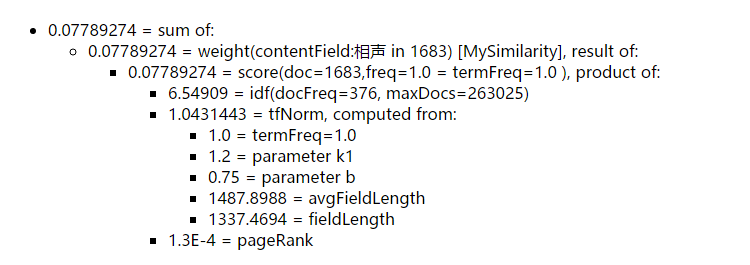
\includegraphics[scale=0.5]{t3}
\caption{排名第三的得分情况}
\end{figure}

\newpage

从得分中我们可以看出,排名第一、第二的网站之所以得分较高,是因为其在标题(titleField)中出现了关键词,且titleField设置的权值为6,因此总得分较高;而由于第三名标题中没有出现关键词,尽管其正文中出现次数很多,正文得分高于前两名的正文得分,但总分却没有前二者高。当然,由于第三名网页Page Rank值较高(是前两名的近百倍),所以排名也比较靠前。

\section{实验总结}

通过这次实验,我们掌握了搜索引擎的基本架构和重要实现,通过自己完成搜索引擎四个子系统,我们对每个子系统的功能和架构有了更深的理解。在实验过程中,我们曾遇到爬取速度太慢、UTF-8编码问题、得分公式不够优、搜索结果不好等问题,但最终都在同学的启发下得以克服。总之,我们在这次实验中收获颇丰,更好地理解了课堂上所讲的原理知识。

\end{document}
